% !TEX root = ./rapport.tex
\chapter{Sprints 1 et 2~: Infrastructure et Gestion des Employés}

\noindent\textbf{Plan}
\begin{enumerate}
  \item Introduction
  \item Sprint 1~: Initialisation et infrastructure de base
  \item Sprint 2~: Gestion des employés
  \item Conclusion
\end{enumerate}

% ─────────────────────────────────────────────────────────────
\section{Introduction}
% ─────────────────────────────────────────────────────────────

Cette première release établit les fondations techniques de la plateforme Synapse.
Le sprint 1 met en place l’architecture microservices, le serveur d’identité Keycloak
et le schéma de base de données Oracle. Le sprint 2 s’appuie sur ces fondations pour
livrer le premier module métier~: l'administration complète du personnel
avec synchronisation bidirectionnelle Oracle--Keycloak.

% ─────────────────────────────────────────────────────────────
\section{Sprint 1~: Initialisation et infrastructure de base}
% ─────────────────────────────────────────────────────────────

\subsection{Objectifs du sprint}

Le sprint~1 constitue le fondement technique de la plateforme Synapse. Avant tout
développement fonctionnel, il est indispensable d’établir l’infrastructure
d’authentification centralisée, le schéma Oracle versionné par Flyway et
l’architecture à sept microservices. Ce sprint répond à la question~: comment
mettre en place un socle de sécurité uniforme (RBAC à six rôles Keycloak)
sur lequel chaque service s’appuiera tout au long du projet~? La durée est de
\textbf{2 semaines} (02--15 fév. 2026).

\begin{table}[H]
\centering
\caption{Objectifs du sprint 1}
\label{tab:sprint1_obj}
\begin{tabularx}{\textwidth}{VlVLVlV}
\rowcolor{headerblue!55}
\hline
\textbf{Tâche} & \textbf{Objectif} & \textbf{Estim.} \\
\hline
Architecture microservices & Créer les sept squelettes de microservices Spring Boot et configurer le POM parent & 2j \\
\hline
Keycloak 26 & Déployer le serveur d’identité, configurer le realm Synapse et les six rôles organisationnels & 2j \\
\hline
Oracle 23ai + Flyway & Initialiser le schéma fondateur via les migrations V1 à V4~: core RH (V1), projets/évaluations (V2), demandes RH (V3), communication (V4) & 2j \\
\hline
Sécurité JWT & Configurer le \texttt{JwtAuthenticationConverter} commun à tous les services & 1j \\
\hline
Angular 21 & Initialiser le projet frontend avec l’intégration \texttt{keycloak-angular} & 1j \\
\hline
Docker Compose & Définir les conteneurs Oracle, Keycloak, Kafka et Zookeeper & 2j \\
\hline
\end{tabularx}
\end{table}

\subsection{Conception UML}

\subsubsection*{Cas d’utilisation~: S’authentifier}

La figure~\ref{fig:uc_auth} ci-dessous présente le diagramme de cas d’utilisation
raffiné relatif à l’authentification.

% Insert figure: Diagramme de cas d’utilisation raffiné — S’authentifier
\begin{figure}[H]
  \centering
  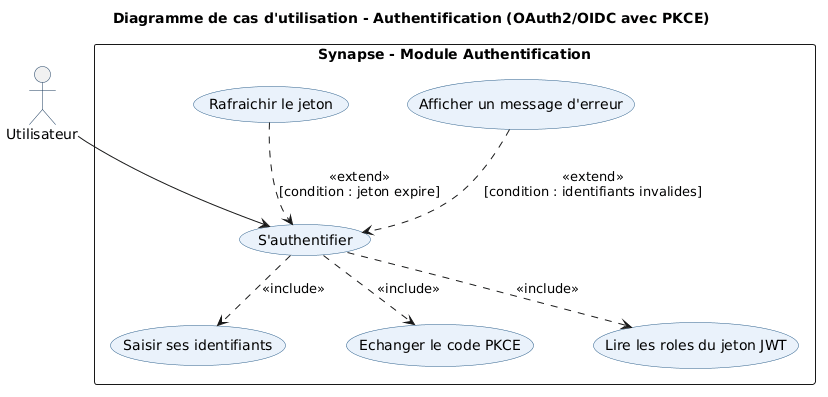
\includegraphics[width=0.90\textwidth,height=0.58\textheight,keepaspectratio]{diagrams/uc_authentifier.png}
  \caption{Diagramme de cas d’utilisation raffiné~: S’authentifier}
  \label{fig:uc_auth}
\end{figure}

La figure~\ref{fig:seq_auth} ci-dessous présente le diagramme de séquence
du cas d’utilisation « S’authentifier ».

\begin{figure}[H]
\centering
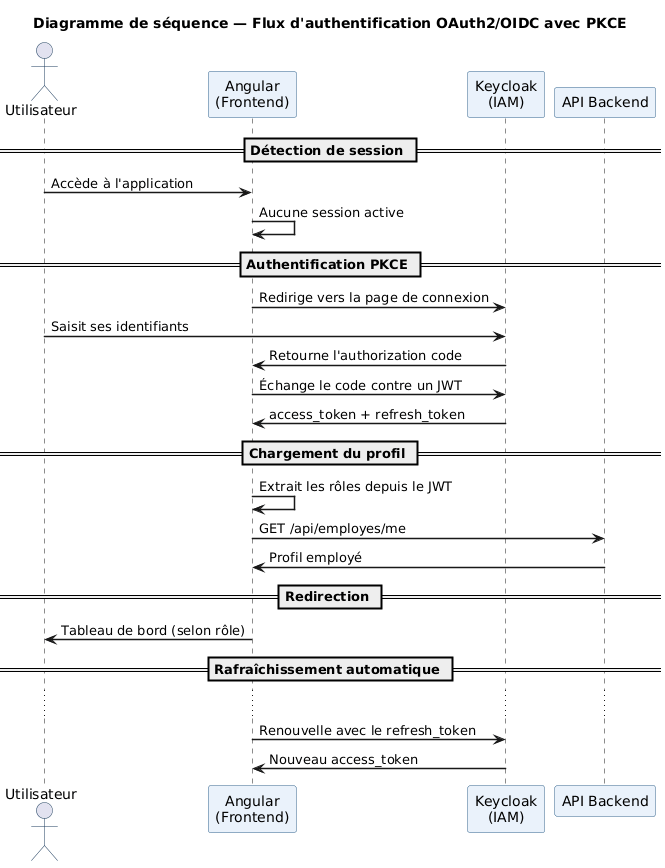
\includegraphics[width=\textwidth,keepaspectratio]{diagrams/seq_authentifier.png}
\caption{Diagramme de séquence~: flux d’authentification OAuth2/OIDC avec PKCE}
\label{fig:seq_auth}
\end{figure}

La table~\ref{tab:uc_auth} ci-dessous présente la description textuelle du cas
d’utilisation « S’authentifier ».

\begin{table}[H]
\centering
\caption{Description textuelle du cas d’utilisation S’authentifier}
\label{tab:uc_auth}
\begin{tabularx}{\textwidth}{VlVLV}
\rowcolor{headerblue!55}
\hline
\textbf{Champ} & \textbf{Description} \\
\hline
Cas d’utilisation & S’authentifier \\
\hline
Acteurs & Tout utilisateur du système (\texttt{ADMIN\_RH}, \texttt{RH}, \texttt{CHEF}, \texttt{EMPLOYE}, \texttt{DIRECTEUR\_GENERAL}, \texttt{COMITE}) \\
\hline
Précondition & L’utilisateur dispose d’un compte actif dans Keycloak \\
\hline
Postcondition & L’utilisateur est authentifié et accède à son tableau de bord selon son rôle \\
\hline
Scénario nominal &
\begin{enumerate}[leftmargin=*,nosep]
  \item L’utilisateur accède à l’application Synapse
  \item Le système détecte l’absence de session et redirige vers la page de connexion
  \item L’utilisateur saisit ses identifiants et valide
  \item Le système vérifie les identifiants et accorde l’accès
  \item L’utilisateur est redirigé vers son tableau de bord selon son profil
\end{enumerate} \\
\hline
Scénarios alternatifs &
\begin{itemize}[leftmargin=*,nosep]
  \item Identifiants incorrects~: message d’erreur, nouvelle tentative possible
  \item Compte inactif~: message « Compte désactivé, contacter l’administrateur »
  \item Session expirée~: reconnexion automatique sans saisie des identifiants
\end{itemize} \\
\hline
\end{tabularx}
\end{table}

\subsection{Implémentation backend}

\begin{table}[H]
\centering
\caption{Composants d'infrastructure partagée — Sprint 1}
\label{tab:infra_sprint1}
\begin{tabularx}{\textwidth}{VlVLVlV}
\rowcolor{headerblue!55}
\hline
\textbf{Composant} & \textbf{Description} & \textbf{Scope} \\
\hline
\texttt{KeycloakJwtRoleConverter} & Extrait \texttt{realm\_access} du JWT et préfixe \texttt{ROLE\_} & Tous microservices \\
\hline
\texttt{SecurityFilterChain} & OAuth2 Resource Server, routes publiques / protégées par rôle & Tous microservices \\
\hline
Flyway V1–V4 & Crée le schéma Oracle~: \texttt{EMPLOYEES}, \texttt{PROJECTS}, \texttt{LEAVE\_REQUESTS}, \texttt{MESSAGES} & Démarrage auto \\
\hline
Docker Compose & Orchestre Oracle~23ai, Keycloak~26, Kafka et Zookeeper & Infrastructure \\
\hline
\end{tabularx}
\end{table}

Le \texttt{KeycloakJwtRoleConverter} est partagé par tous les microservices~: il extrait
les rôles du JWT et les préfixe en \texttt{ROLE\_X} pour que \texttt{@PreAuthorize}
fonctionne nativement sans duplication. Les migrations Flyway V1–V4 initialisent le
schéma Oracle complet au démarrage~; les migrations V5–V11 sont appliquées
progressivement dans les sprints suivants.

\begin{figure}[H]
  \centering
  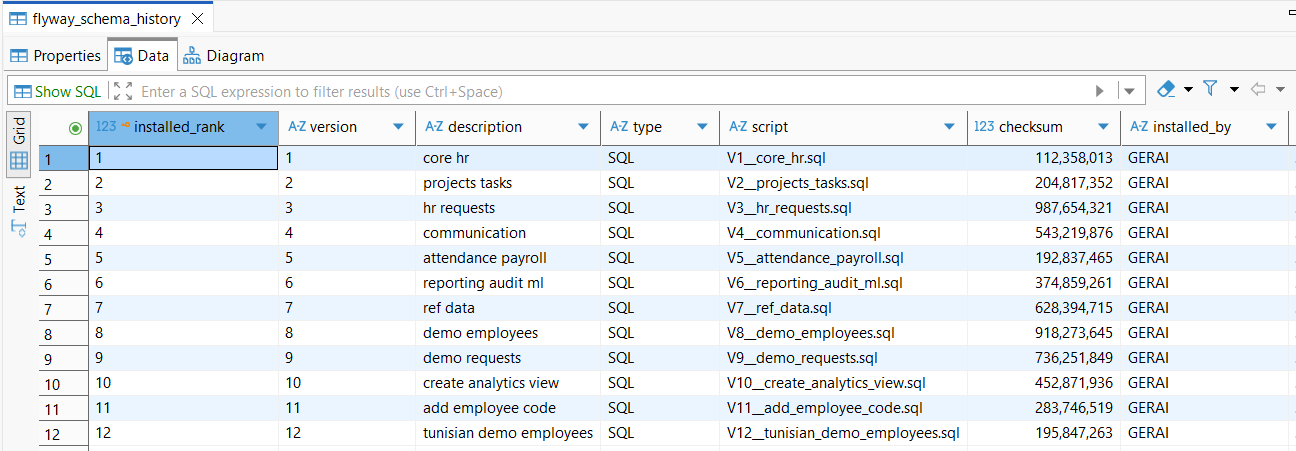
\includegraphics[width=0.88\textwidth,height=0.52\textheight,keepaspectratio]{images/flyway_history.png}
  \caption{Table \texttt{flyway\_schema\_history}~: schéma fondateur V1 à V4 (core RH, projets, demandes, communication)}
  \label{fig:flyway_history}
\end{figure}

\subsection{Implémentation frontend}

\begin{table}[H]
\centering
\caption{Composants Angular — Sprint 1}
\label{tab:angular_sprint1}
\begin{tabularx}{\textwidth}{VlVlVlVLV}
\rowcolor{headerblue!55}
\hline
\textbf{Composant} & \textbf{Route} & \textbf{Rôle} & \textbf{Fonctionnalité} \\
\hline
\texttt{AppComponent} & / & Tous & Shell principal, routage racine, initialisation Keycloak \\
\hline
\texttt{requireRoleGuard} & Toutes routes protégées & Tous & Vérification du rôle JWT~; redirection si accès refusé \\
\hline
\texttt{BearerInterceptor} & — & Tous & Injection automatique du token JWT dans chaque requête \texttt{HttpClient} \\
\hline
\texttt{DashboardRedirectComponent} & /dashboard & Tous & Redirection vers la vue métier selon le rôle (EMPLOYE, CHEF, RH…) \\
\hline
\end{tabularx}
\end{table}

L’intégration de Keycloak dans Angular 21 est réalisée via \texttt{keycloak-angular~21}\textsuperscript{[5]}~:
l’application démarre uniquement après l’initialisation de Keycloak dans \texttt{main.ts}.
Le \texttt{requireRoleGuard} vérifie le rôle du token JWT sur chaque route protégée~;
le \texttt{BearerInterceptor} injecte le token sur toutes les requêtes sortantes.

\subsection{Interfaces de l’application}

La figure~\ref{fig:login_page} présente la page de connexion générée par Keycloak,
et la figure~\ref{fig:keycloak_console} la console d’administration montrant le realm
Synapse et ses six rôles.

\begin{figure}[H]
  \centering
  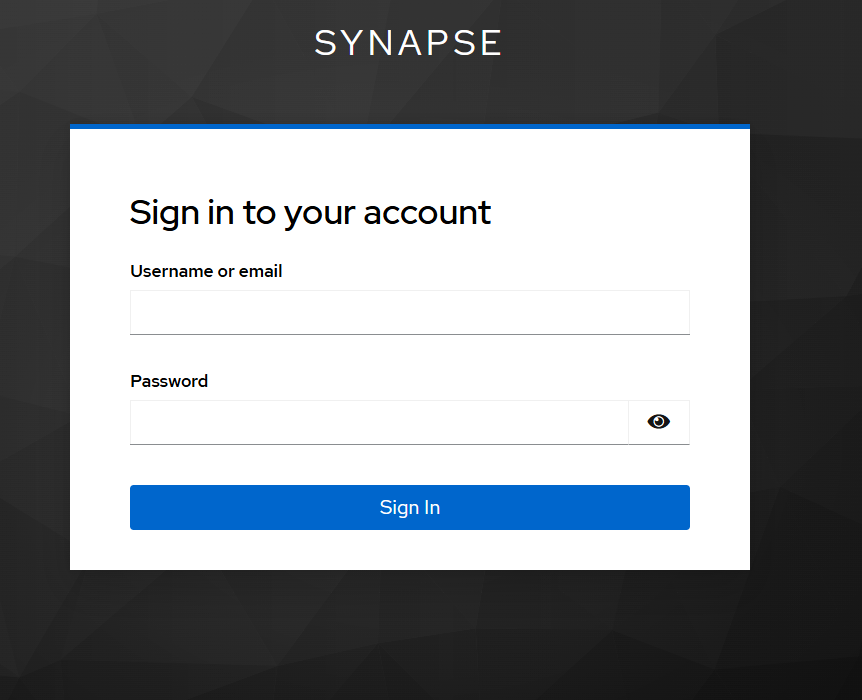
\includegraphics[width=0.82\textwidth,height=0.46\textheight,keepaspectratio]{images/screenshot_login.png}
  \caption{Page de connexion de la plateforme Synapse}
  \label{fig:login_page}
\end{figure}

\begin{figure}[H]
  \centering
  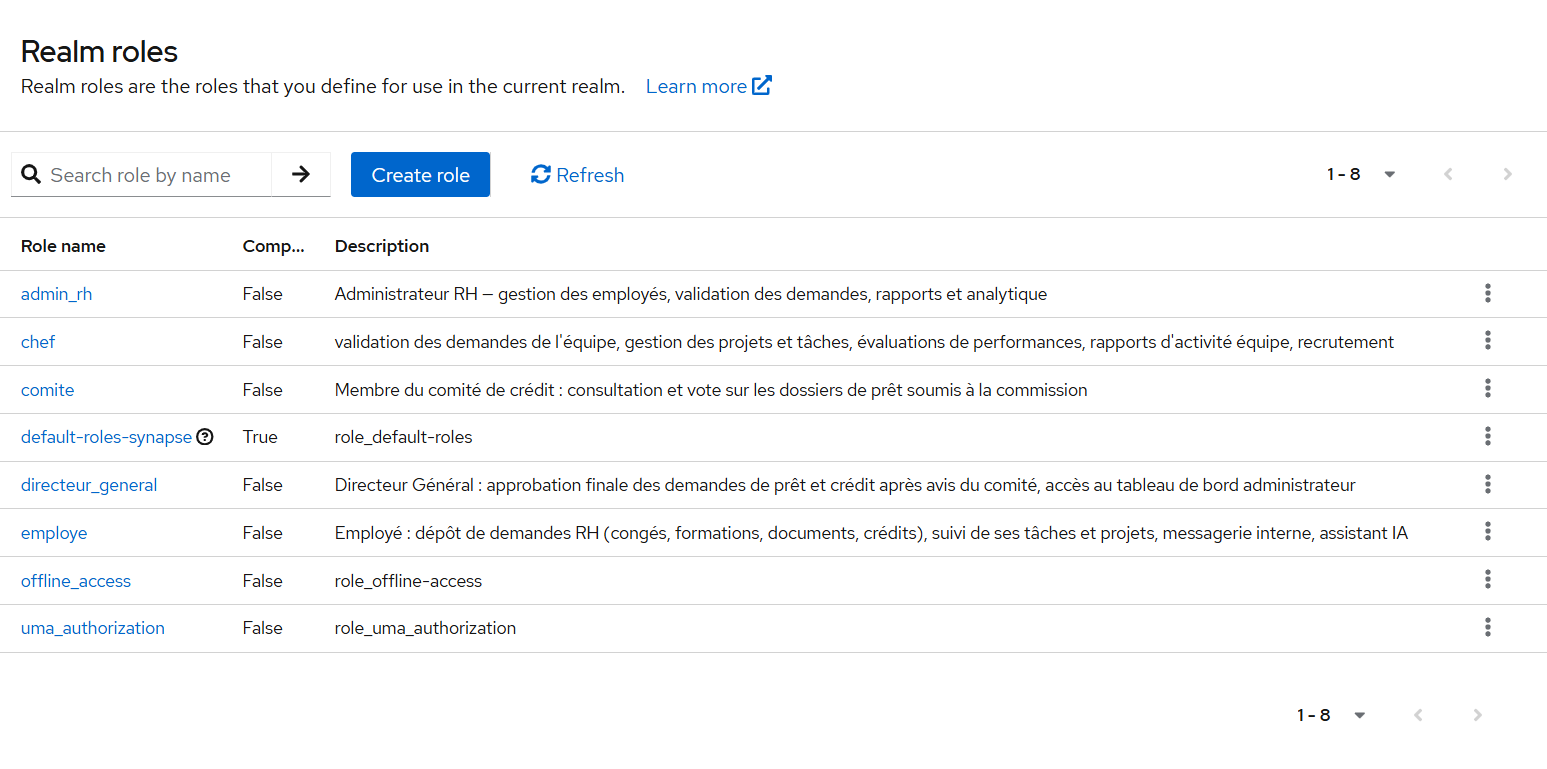
\includegraphics[width=0.82\textwidth,height=0.46\textheight,keepaspectratio]{images/keycloak_admin_realm.png}
  \caption{Console d’administration Keycloak~: realm Synapse et rôles organisationnels}
  \label{fig:keycloak_console}
\end{figure}

\subsection{Sprint review}

Le tableau~\ref{tab:sprint1_review} présente les résultats du sprint~1.

\begin{table}[H]
\centering
\caption{Sprint 1 review}
\label{tab:sprint1_review}
\begin{tabularx}{\textwidth}{VLVCVCVCV}
\rowcolor{headerblue!55}
\hline
\textbf{Tâche} & \textbf{Terminé} & \textbf{À améliorer} & \textbf{Inachevé} \\
\hline
Architecture microservices (7 services) & \faCheckCircle & & \\
\hline
Déploiement Keycloak 26 + realm Synapse & \faCheckCircle & & \\
\hline
Migrations Flyway V1--V4 & \faCheckCircle & & \\
\hline
Configuration JWT / RBAC (alignement rôles + robustesse converter) & \faCheckCircle & & \\
\hline
Intégration \texttt{keycloak-angular} & \faCheckCircle & & \\
\hline
Docker Compose (Oracle, Keycloak, Kafka, Zookeeper) & \faCheckCircle & & \\
\hline
\end{tabularx}
\end{table}

\paragraph{Obstacle résolu~: configuration JWT/RBAC.}
Le \texttt{KeycloakJwtRoleConverter} préfixait les rôles en majuscules (\texttt{ROLE\_ADMIN\_RH}) tandis que les \texttt{SecurityFilterChain} utilisaient des libellés en minuscules~; l'uniformisation des identifiants, l'ajout d'une valeur par défaut pour le \texttt{client-id} et le passage du niveau de log des rôles de \texttt{INFO} à \texttt{DEBUG} ont résolu le problème et assaini les traces en production.

% ─────────────────────────────────────────────────────────────
\section{Sprint 2~: Gestion des employés}
% ─────────────────────────────────────────────────────────────

\subsection{Objectifs du sprint}

Le sprint~2 livre le premier incrément fonctionnel utilisable de Synapse~: la
administration complète du personnel. Il répond à la problématique
métier centrale~: comment créer un compte employé de manière atomique, en
synchronisant Oracle et Keycloak en une seule opération~? Sans ce sprint, aucun
utilisateur ne peut accéder à la plateforme. La durée est de \textbf{2 semaines}
(16 fév.--01 mars 2026).

\begin{table}[H]
\centering
\caption{Objectifs du sprint 2}
\label{tab:sprint2_obj}
\begin{tabularx}{\textwidth}{VlVLVlVlV}
\rowcolor{headerblue!55}
\hline
\textbf{Tâche} & \textbf{Objectif} & \textbf{US} & \textbf{Estim.} \\
\hline
employe-service (CRUD) & Créer, modifier, désactiver un employé depuis l’interface admin & US-01, 02, 03 & 3j \\
\hline
Synchronisation Oracle--Keycloak & Provisionner automatiquement le compte Keycloak lors de la création d’un employé & US-01 & 2j \\
\hline
Génération de matricule & Produire un code unique au format \texttt{EMP-XXXX} à chaque création & US-01 & 1j \\
\hline
Notifications e-mail & Envoyer un e-mail de bienvenue avec lien de connexion via MailHog & US-01 & 1j \\
\hline
Interface admin Angular & Formulaire de création, liste avec filtres, fiche de profil & US-04, US-05 & 3j \\
\hline
\end{tabularx}
\end{table}

\subsection{Conception UML}

\subsubsection*{Cas d’utilisation~: Gérer les employés}

La figure~\ref{fig:uc_employe} ci-dessous présente le diagramme de cas d’utilisation
raffiné relatif à la gestion des employés.

% Insert figure: Diagramme de cas d’utilisation raffiné — Gérer les employés
\begin{figure}[H]
  \centering
  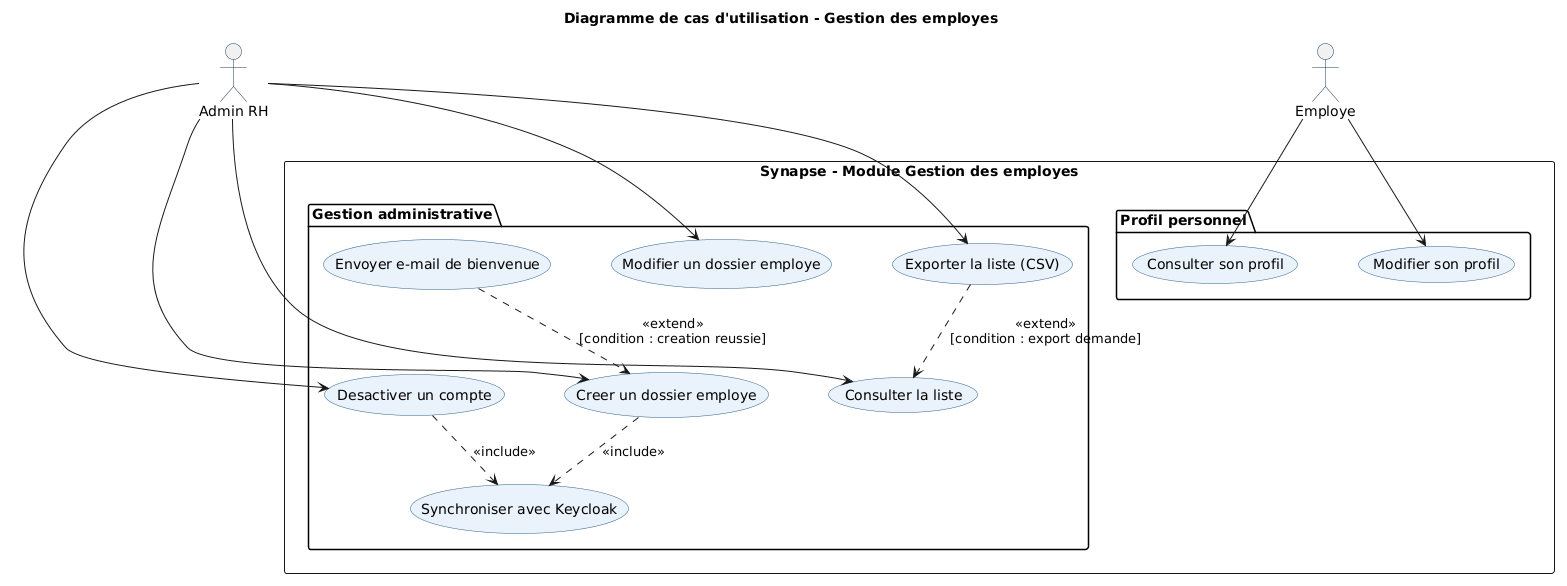
\includegraphics[width=0.90\textwidth,height=0.58\textheight,keepaspectratio]{diagrams/uc_gerer_employes.png}
  \caption{Diagramme de cas d’utilisation raffiné~: gérer les employés}
  \label{fig:uc_employe}
\end{figure}

La figure~\ref{fig:seq_create_emp} ci-dessous présente le diagramme de séquence du
cas d’utilisation « Créer un employé ».


\begin{figure}[H]
\centering
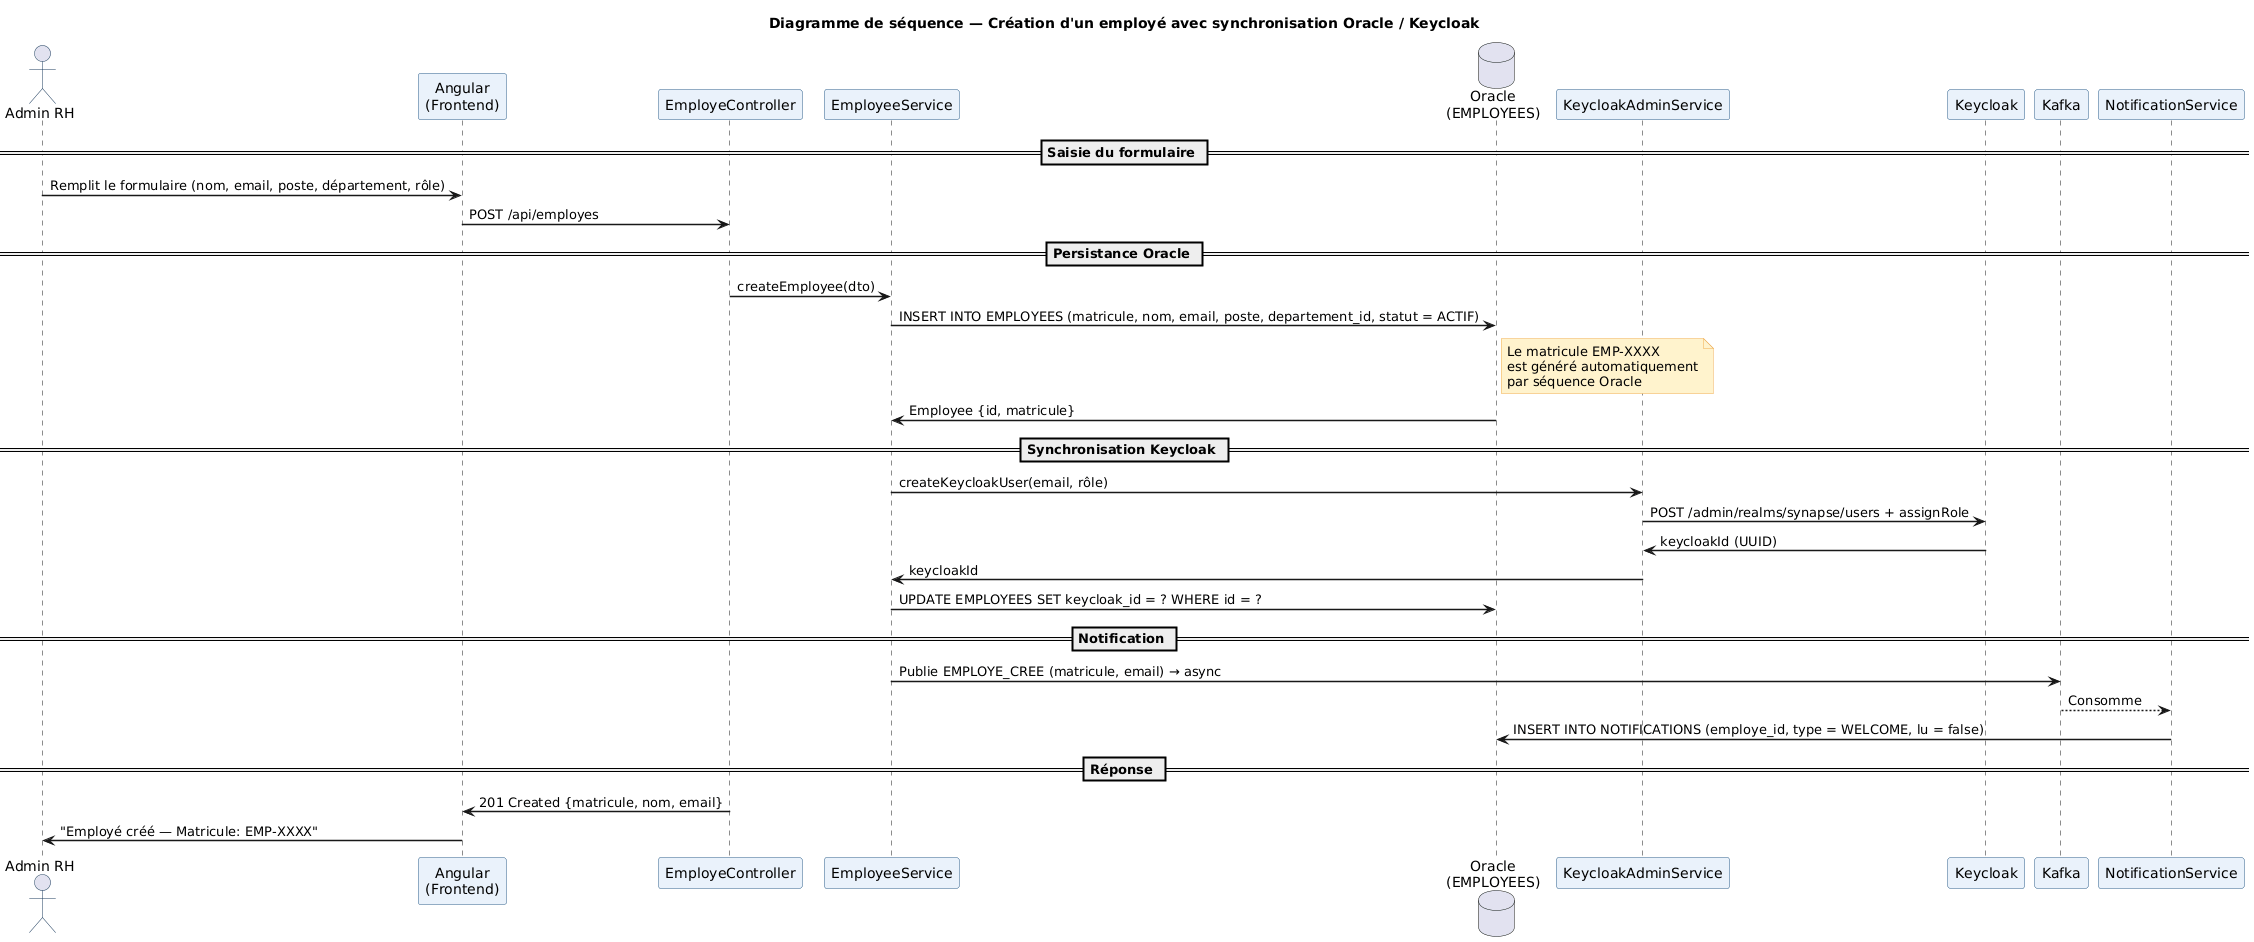
\includegraphics[width=\textwidth,height=0.50\textheight,keepaspectratio]{diagrams/sequence_creer_employe.png}
\caption{Diagramme de séquence~: création d’un employé avec synchronisation Oracle--Keycloak}
\label{fig:seq_create_emp}
\end{figure}


La table~\ref{tab:uc_create_emp} ci-dessous présente la description textuelle du cas
d’utilisation « Créer un employé ».

\begin{table}[H]
\centering
\caption{Description textuelle du cas d’utilisation Créer un employé}
\label{tab:uc_create_emp}
\begin{tabularx}{\textwidth}{VlVLV}
\rowcolor{headerblue!55}
\hline
\textbf{Champ} & \textbf{Description} \\
\hline
Cas d’utilisation & Créer un employé \\
\hline
Acteur & Administrateur RH (\texttt{ADMIN\_RH}) \\
\hline
Précondition & L’administrateur est authentifié et accède à l’interface de gestion des employés \\
\hline
Postcondition & Compte créé dans Oracle et Keycloak~; matricule généré~; e-mail de bienvenue envoyé \\
\hline
Scénario nominal &
\begin{enumerate}[leftmargin=*,nosep]
  \item L’administrateur remplit le formulaire (nom, prénom, département, poste, e-mail)
  \item Le système valide les données et génère automatiquement un matricule unique
  \item Un compte d’accès à la plateforme est créé avec le rôle approprié
  \item Un e-mail de bienvenue avec lien de connexion est envoyé à l’employé
\end{enumerate} \\
\hline
Scénarios alternatifs &
\begin{itemize}[leftmargin=*,nosep]
  \item E-mail déjà existant~: message « Adresse e-mail déjà utilisée »
  \item Erreur lors de la création du compte d’accès~: le dossier employé est enregistré~; l’administrateur peut relancer la création du compte ultérieurement
  \item Champ obligatoire manquant~: message de validation avant soumission
\end{itemize} \\
\hline
\end{tabularx}
\end{table}

\subsection{Implémentation backend}

\paragraph{Génération du matricule \texttt{EMP-XXXX}.}
À chaque création d'employé, le service génère automatiquement un code matricule
unique au format \texttt{EMP-XXXX}. La logique repose sur une requête Oracle qui
récupère la valeur maximale des matricules existants (\texttt{MAX(employee\_code)}),
en extrait le suffixe numérique, l'incrémente et formate le résultat avec un
\textit{zero-padding} sur quatre chiffres (\texttt{String.format("EMP-\%04d", n)}).
La valeur est générée côté applicatif dans une transaction, garantissant l'unicité
par la contrainte \texttt{UNIQUE} de la colonne \texttt{employee\_code}.

\begin{table}[H]
\centering
\caption{Principaux endpoints REST de l'\textit{employe-service}}
\label{tab:api_employe}
\begin{tabularx}{\textwidth}{VlVlVLVlV}
\rowcolor{headerblue!55}
\hline
\textbf{Méthode} & \textbf{Endpoint} & \textbf{Description} & \textbf{Rôle requis} \\
\hline
POST & \texttt{/employees} & Créer un employé (matricule auto, sync Keycloak) & ADMIN\_RH \\
\hline
GET & \texttt{/employees} & Lister les employés (filtres statut, département) & RH, ADMIN\_RH, CHEF \\
\hline
GET & \texttt{/employees/\{id\}} & Consulter une fiche employé & Tous \\
\hline
PUT & \texttt{/employees/\{id\}} & Modifier un employé (poste, département, photo) & ADMIN\_RH \\
\hline
DELETE & \texttt{/employees/\{id\}} & Désactiver un employé (révocation Keycloak) & ADMIN\_RH \\
\hline
GET & \texttt{/employe/profil} & Consulter sa propre fiche (contrat, documents) & EMPLOYE \\
\hline
POST & \texttt{/employe/documents} & Téléverser un document RH personnel & EMPLOYE \\
\hline
GET & \texttt{/equipe/membres} & Liste filtrée de l'équipe d'un chef & CHEF \\
\hline
\end{tabularx}
\end{table}


\begin{figure}[H]
  \centering
  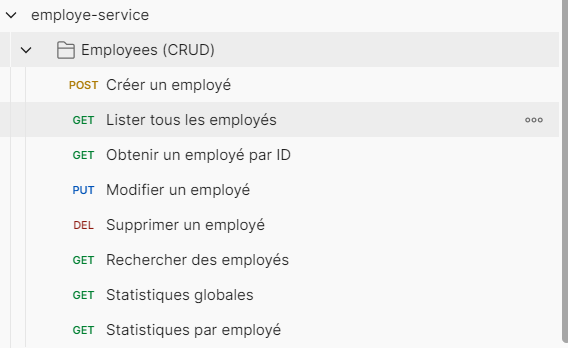
\includegraphics[width=0.88\textwidth,height=0.52\textheight,keepaspectratio]{images/apis_employe_service.png}
  \caption{APIs REST de l'\textit{employe-service}~: endpoints CRUD}
  \label{fig:apis_employes}
\end{figure}

\subsection{Implémentation frontend}

\begin{table}[H]
\centering
\caption{Composants Angular — Sprint 2}
\label{tab:angular_sprint2}
\begin{tabularx}{\textwidth}{VlVlVlVLV}
\rowcolor{headerblue!55}
\hline
\textbf{Composant} & \textbf{Route} & \textbf{Rôle} & \textbf{Fonctionnalité} \\
\hline
\texttt{EmployeListComponent} & /admin/employes & ADMIN\_RH, RH & Liste filtrée par statut et département, actions CRUD \\
\hline
\texttt{EmployeFormComponent} & /admin/employes/new & ADMIN\_RH & Formulaire de création avec matricule auto et affectation département \\
\hline
\texttt{ProfilEmployeComponent} & /profil & EMPLOYE & Consultation de la fiche personnelle, contrat et documents \\
\hline
\texttt{EquipeComponent} & /chef/equipe & CHEF & Vue filtrée des membres de l’équipe managée \\
\hline
\end{tabularx}
\end{table}

Les composants standalone utilisent la stratégie \texttt{OnPush}. \texttt{EmployeService}
communique via \texttt{HttpClient}~; le \texttt{BearerInterceptor} injecte le JWT sur
chaque requête. \texttt{EquipeComponent} consomme \texttt{/equipe/membres}~: le filtrage
est appliqué côté backend selon l’identité du chef connecté.

\subsection{Interfaces de l’application}

Les figures ci-dessous présentent les principales interfaces de la gestion des employés~:
liste filtrée, fiche de profil et tableau de bord administrateur. Le formulaire de création
est présenté en Annexe~I (voir figure~\ref{fig:create_emp_form}).

\begin{figure}[H]
  \centering
  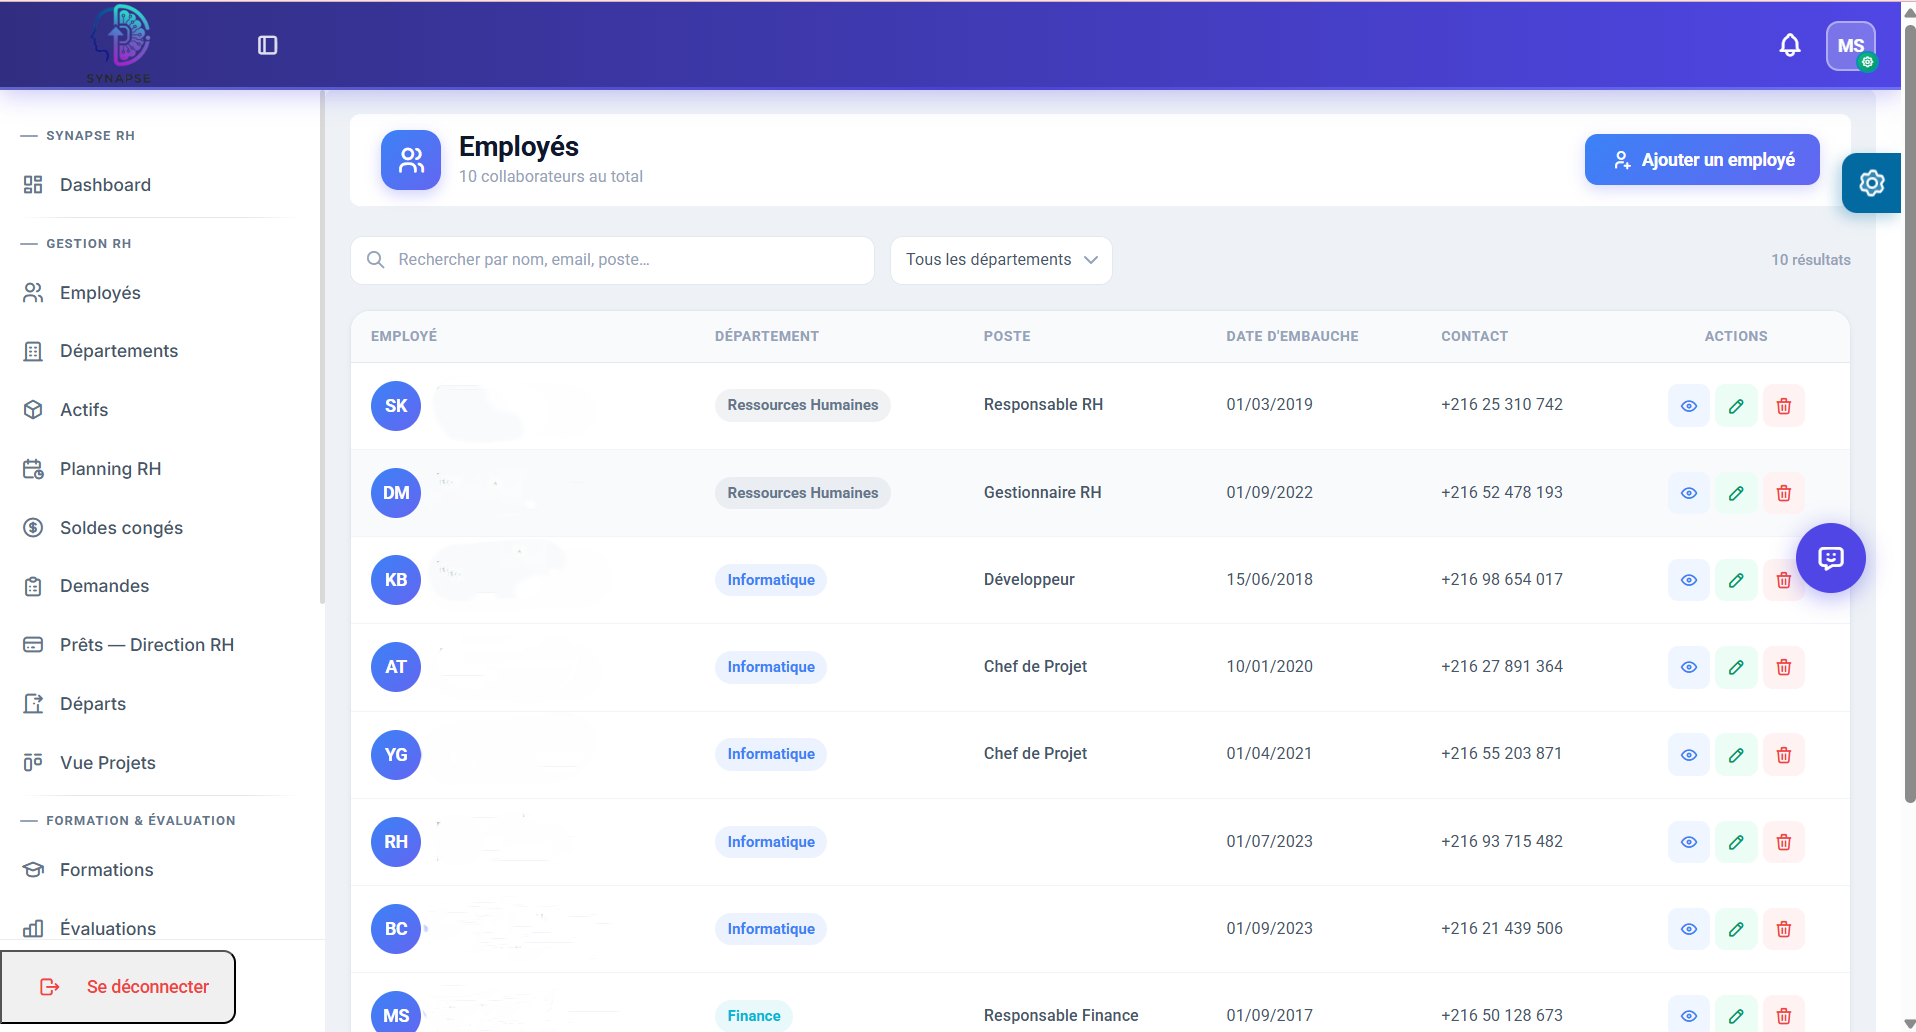
\includegraphics[width=0.82\textwidth,height=0.46\textheight,keepaspectratio]{images/screenshot_employee_list.png}
  \caption{Liste des employés~: filtrage par département, statut et actions rapides}
  \label{fig:employee_list}
\end{figure}

\begin{figure}[H]
  \centering
  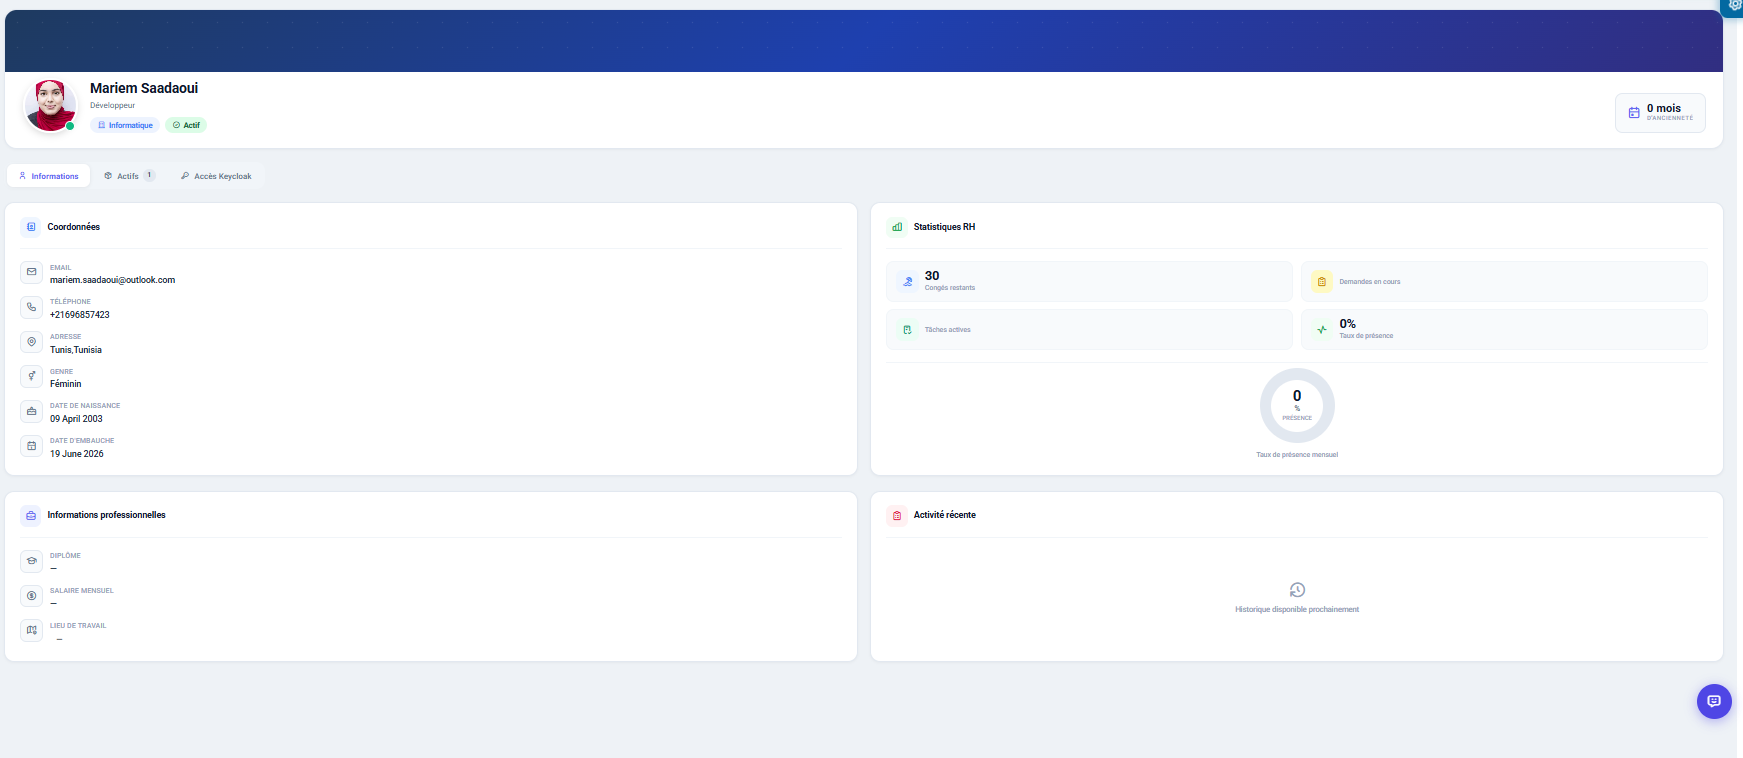
\includegraphics[width=0.82\textwidth,height=0.46\textheight,keepaspectratio]{images/screenshot-employee_profile.png}
  \caption{Fiche de profil d’un employé~: informations, documents et historique}
  \label{fig:employee_profile}
\end{figure}

\subsection{Sprint review}

Le tableau~\ref{tab:sprint2_review} présente les résultats du sprint~2.

\begin{table}[H]
\centering
\caption{Sprint 2 review}
\label{tab:sprint2_review}
\begin{tabularx}{\textwidth}{VLVCVCVCV}
\rowcolor{headerblue!55}
\hline
\textbf{Tâche} & \textbf{Terminé} & \textbf{À améliorer} & \textbf{Inachevé} \\
\hline
employe-service (CRUD complet) & \faCheckCircle & & \\
\hline
Synchronisation Oracle--Keycloak & \faCheckCircle & & \\
\hline
Génération automatique du matricule & \faCheckCircle & & \\
\hline
Notifications e-mail (MailHog) & \faCheckCircle & & \\
\hline
Interface Angular~: liste, création, profil & \faCheckCircle & & \\
\hline
Tableau de bord administrateur & \faCheckCircle & & \\
\hline
Gestion des départs (fiches de départ + désactivation Keycloak) & \faCheckCircle & & \\
\hline
\end{tabularx}
\end{table}

\paragraph{Obstacle résolu~: synchronisation Oracle--Keycloak.}
Maintenir la cohérence entre la base Oracle et le référentiel Keycloak sans transaction distribuée a été le principal défi du sprint~2~: chaque création ou départ d'employé devait déclencher un appel REST à l'API Keycloak Admin via une couche service dédiée, garantissant l'atomicité métier et évitant les états incohérents en cas d'échec réseau.

% ─────────────────────────────────────────────────────────────
\section{Conclusion}
% ─────────────────────────────────────────────────────────────

Cette première release a établi le socle technique de Synapse~: serveur d’identité
centralisé, schéma de données versionné et synchronisation Oracle--Keycloak
opérationnelle. Ces fondations garantissent que tous les microservices suivants
bénéficient d’une authentification uniforme et d’un RBAC cohérent, sans duplication
de logique de sécurité. Le sprint~2 a validé ce socle en livrant le premier module
métier complet, de la création en base à l’envoi de l’e-mail de bienvenue.
